\documentclass[10pt,twocolumn,letterpaper]{article}

\usepackage{cvpr}
\usepackage{times}
\usepackage{epsfig}
\usepackage{graphicx}
\usepackage{amsmath}
\usepackage{amssymb}
\usepackage{svg}

% Include other packages here, before hyperref.

% If you comment hyperref and then uncomment it, you should delete
% egpaper.aux before re-running latex.  (Or just hit 'q' on the first latex
% run, let it finish, and you should be clear).
\usepackage[pagebackref=true,breaklinks=true,letterpaper=true,colorlinks,bookmarks=false]{hyperref}

%\cvprfinalcopy % *** Uncomment this line for the final submission

\def\cvprPaperID{****} % *** Enter the CVPR Paper ID here
\def\httilde{\mbox{\tt\raisebox{-.5ex}{\symbol{126}}}}

% Pages are numbered in submission mode, and unnumbered in camera-ready
\ifcvprfinal\pagestyle{empty}\fi
\begin{document}

%%%%%%%%% TITLE
\title{Convolutional Neural Network to Detect Equivalent Questions in Online Forums  \\ DL-IC 2018 Project} 

\author{Luca Scannapieco\\
Politecnico di Milano\\
{\tt\small luca.scannapieco@mail.polimi.it}
% For a paper whose authors are all at the same institution,
% omit the following lines up until the closing ``}''.
% Additional authors and addresses can be added with ``\and'',
% just like the second author.
% To save space, use either the email address or home page, not both
\and
Nicola Sosio\\
Politecnico di Milano\\
{\tt\small nicola.sosio@mail.polimi.it}
\and
Maria Chiara Zaccardi\\
Politecnico di Milano\\
{\tt\small mariachiara.zaccardi@mail.polimi.it}
}

\maketitle
%\thispagestyle{empty}

%%%%%%%%% ABSTRACT
\begin{abstract}
   In the context of online forums, although two questions may seem very different in terms of vocabulary, length and syntax, they may eventually ask the same thing. In this work, we try to detect semantically equivalent questions using a simple Convolutional Neural Network (CNN). The proposed CNN generates distributed vector representations for pairs of questions and score them using a similarity metric. This work is the replication of \cite{bogdanova2015detecting}: we basically try to perform the same experiments and compare our results with theirs. The replication is made harder by the fact that some crucial implementation details are missing in the Bogdanova et al.'s description. Hence, we find quite stimulating to replicate this paper filling the holes with our own ideas. In particular, our efforts focus mainly on the following three aspects that were not explicitly treated in the paper: unequal text length, the type of convolution and the training of in-domain word embeddings. \\
Moreover, we attempt to make the simple modification to the network, suggested by Kim \cite{kim2014convolutional}. This simple change increases the validation accuracy by about 1\%. \\
The final results are quite close to our target; even the optimal hyper-parameters values of the network are very similar to the ones in \cite{bogdanova2015detecting}. It is worth clarifying that, since we use domain-specific data for both training and testing the model, the obtained performances are guaranteed to hold only for pairs of questions coming from that specific domain.
\end{abstract}

%%%%%%%%% BODY TEXT
%------------------------------------------------------------------------
\section{Introduction}
Natural Language Processing (NLP) is just one of several fields emerging from Artificial Intelligence. In NLP we want the machine to process and analyze large amount of natural language data to accomplish very interesting tasks (such as Sentiment Analysis, Language Identification and many others). Nowadays, these tasks are plenty and many works on them has been already carried out \footnote{Here is a very interesting repository collecting several NLP tasks along with their main references: \\ \url{https://github.com/Kyubyong/nlp_tasks}}. In this paper, we focus on the task of predicting whether two questions from an online forum are semantically equivalent, i.e. they can be answered by the exact same answer. This can be a very useful tool for Question-Answering community sites as they typically want to keep their databases as less redundant as possible, so to make the searches of their users both faster and more effective. Furthermore, they want to keep people from wasting their time in answering already solved questions. \\
The main contribution of this work is \cite{bogdanova2015detecting}. In their work, Bogdanova et al. propose a simple Convolutional Neural Network (CNN) to detect semantically equivalent questions. The proposed network first transforms words into \emph{word embeddings} and then applies a convolutional layer which generates question-wide vectors representations. Finally, pairs of questions are scored using a similarity function. The most interesting experimental result is the evaluation of in-domain word embeddings against the word embeddings generated using all of the English Wikipedia. In particular, they show that domain-specific word embeddings achieve higher performances. \\
In general, both validations accuracy and optimal hyper-parameter values obtained by our implementation are very close to the ones of the replicated paper.\\
The authors of \cite{bogdanova2015detecting} accurately describe the architecture of the network, but many crucial details of the model are missing in their description. Hence, we find quite stimulating to replicate this paper filling the holes with our own ideas. In particular, our efforts focus mainly on four aspects that are not explicitly treated in \cite{bogdanova2015detecting}. In the following we just introduce them; they are further analyzed in Section 3.
    \paragraph{Handling questions of different sizes.}
    Bogdanova et al. explicitly state that the different sizes of questions is one of the main challenges of their work. Nevertheless, they do not specify the way they solved this issue. We, therefore, try to fix the length of each question to the \textbf{maximum} and to the \textbf{mean} length of all the questions. The first approach does yield the greatest accuracy.
    \paragraph{The type of convolution.}
    For the implementation of our network we use a 1-dimensional convolution. Indeed, text can be seen as images with the input maps having only one dimension (height, without width) corresponding to the question length and where the number of input maps is nothing but the size of the word embeddings. The type of convolution represents another missing detail of \cite{bogdanova2015detecting}.    
    \paragraph{The training of in-domain word embeddings.}
    The paper \cite{bogdanova2015detecting} does not provide any information about the model adopted to train in-domain word embeddings. Initially, we tried to build our own \emph{word2vec skip-gram} model \cite{mikolov2013distributed} trained with the same dataset employed to train the main network \footnote{To do so we followed this good tutorial: \url{http://adventuresinmachinelearning.com/word2vec-keras-tutorial/}}. However, the training of this network turned out to be very slow and the resulting embeddings performed poorly. \\
    We, then, decided to use Gensim \footnote{\url{https://radimrehurek.com/gensim/index.html}}, a very simple library which generates word-embeddings given the training data. The resulting embeddings perform very well, allowing the main network to achieve up to 90\% of accuracy on the validation set.
    	\paragraph{CNN Multi-channel}
    	As suggested by Kim in \cite{kim2014convolutional}, we also investigate a simple variant of the CNN proposed in \cite{bogdanova2015detecting}. The first hidden layer of this network has two ``channels'' of word-embeddings: one that is kept static during training and one that is fine-tuned via backpropagation. This modification brings an improvement of around 1\% to the performances of the network.  


%------------------------------------------------------------------------
\section{Related work}
Detecting text similarities is a problem which was probably born before deep learning. In \cite{gomaa2013survey}, Gomaa et al. survey existing algorithms for both lexical and semantical text similarity. All these algorithms have nothing to do with Neural Networks, and can therefore be used as baselines to understand how much deep learning has improved the state-of-the-art.\\
In \cite{kim2014convolutional}, Kim proposes a very simple CNN architecture trained on top of pre-trained word vectors. He experiments the same network on 7 different sentence-level classification tasks and, for each task, he compares the obtained results with the state-of-the-art: the CNN approach improves upon the state-of-the-art on 4 out of 7 tasks. Moreover, he proposes a slight modification of the network with 2 channels of word vectors: one that is kept static during the training and one that is fine-tuned via backpropagation. Although not explicitly stated, we think this is the main contribution of \cite{bogdanova2015detecting} as the network architecture is pretty much the same. The Kim's architecture represents the state-of-the-art on many NLP sentence classification tasks and it is often used as a layer of more complex networks which need to compute sentence-level distributed vectors representation. For example, in \cite{severyn2015learning}, the network is used as a fundamental preprocessing step in a learning-to-rank algorithm. \\
A different but still interesting approach to the problem of text classification, is described in \cite{zhang2015character}. In this article, the authors explore treating text as a kind of raw signal at character level, and applying temporal (1-dimensional) Convolutional Network to it.\\
Different CNN architectures are used for solving a wide range of NLP tasks and many encouraging results have been already achieved. Yih et al. \cite{yih2014semantic} introduce a novel semantic similarity model based on a CNN architecture for the task of answering single-relation factual questions. Hu et al. \cite{hu2014convolutional} propose a CNN architecture for hierarchical sentence modeling and sentence matching. Convolution is also used by Dos Santos et al. \cite{dos2014deep} for sentiment analysis of short texts that jointly uses character-level, word-level and sentence-level information.\\
To tackle the problem of sentences with different lengths, Socher et al. \cite{socher2011dynamic}, introduce a novel dynamic pooling layer which computes a fixed-sized representation from the variable-sized matrices. Another approach could be to use Long Short-Term Memory (LSTM), generating fixed-sized states from the input sentences (as done in \cite{tai2015improved}).\\
In \cite{zhou2015c}, a novel model called C-LSTM is presented: this model stack CNN and LSTM in a unified architecture for semantic sentence modeling. In this way, they are able to combine the strengths of both architectures. In particular, they apply CNN to text data and feed consecutive window features directly to LSTM. In this way, their architecture enables LSTM to learn long-range dependencies from higher-order sequential features.
%------------------------------------------------------------------------
\section{Proposed approach}
In this section we present our strategy for detecting semantically equivalent questions. In Subsection 3.1, we describe in detail the architecture of the Neural Network. Then, in subsequent subsections, we focus on the decisions we have made about the aspects left unspecified by Bogdanova et al.
%-------------------------------------------------------------------------
\subsection{Neural Network Architecture}
As detailed in Figure \ref{fig:network}, the inputs for the network are tokenized text strings of the two questions. In the first step, the CNN transforms words into real valued feature vectors, also known as \emph{word embeddings}. Next, a convolutional layer is used to construct two distributed vector representations $\vec{r}_{q_1}$ and $\vec{r}_{q_2}$, one for each input question. Finally, the CNN computes a similarity score between $\vec{r}_{q_1}$ and $\vec{r}_{q_2}$. Pairs of questions with similarity above a threshold are considered duplicates. Each of these step is explained in more details in the following.
\begin{figure}[t]
\begin{center}
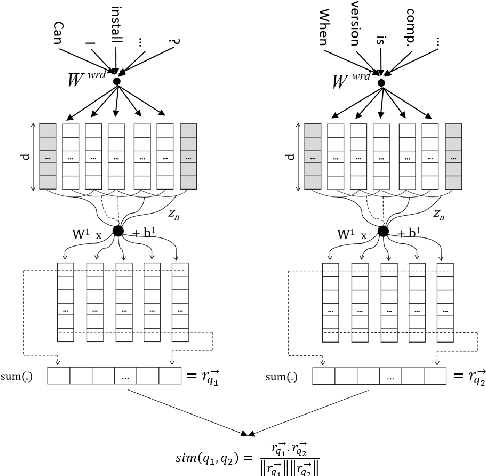
\includegraphics[width=0.8\linewidth]{img/network.png}
\end{center}
\caption{The network architecture.}
\label{fig:network}
\end{figure}

\subsubsection{From text to embeddings}
The first layer of the network transforms words into representations that capture syntactic and semantic information about the words. The initialization of this layer requires two strictly correlated objects:
\begin{itemize}
\item \textbf{The vocabulary}: a dictionary $V$ associating each word of the corpora used to train the embeddings to an integer index. In this vocabulary, we must also reserve an index for all the words which are not present in the vocabulary itself. Best practices suggest to have the index $0$ for the \emph{unknown} words and then having the other indexes ordered by most common words.
\item \textbf{The pre-trained word-embeddings}: a matrix $W_0 \in \mathbb{R}^{|V| \times d}$ where $d$ is the size of the word embeddings. In this matrix, the $i$-th row corresponds to the word embedding of the $i$-th word in the vocabulary.
\end{itemize}
The input of this layer is a 1-dimensional vector $\vec{q}=[w_1, w_2, ... , w_N]$ where the element $w_i$ is an integer number corresponding to the index of the $i$-th word of the question. We initialize the layer with our pre-trained word embeddings \footnote{either the word embeddings trained by us or the those trained by Google}, which is the matrix $W_0$. This layer, for each index $w_i$ of the input vector, retrieves the corresponding vector representation $\vec{r}^{w_i}$ in matrix $W_0$. Hence, the output is a matrix $X_0 \in \mathbb{R}^{N \times d}$.\\
In the simplest implementation of the network, the matrix $W_0$ is kept static during the training. In Section \ref{multichannel} we describe a simple modification in which this matrix becomes trainable.\\
Notice that using pre-trained word embeddings, implies that the values of both the $d$ and $|V|$ have been already decided by those who trained the matrix $W_0$.

\subsubsection{The convolution}
We use a convolutional layer to compute the question-wide distributed vector representations $\vec{r}_{q_1}$ and $\vec{r}_{q_2}$. For each question, the convolutional layer first produces local features around each word in the question. Then, it combines these local features using a sum operation to create a fixed-sized feature vector (representation) for the question.\\
Given a question $q$, the convolutional layer applies a matrix-vector operation to each window of size $k$ of successive windows in $\vec{q}_{emb} = [\vec{r}^{w_1},\vec{r}^{w_2}, ..., \vec{r}^{w_N}]$. Let us define the vector $\vec{z}_n \in \mathbb{R}^{dk}$ as the concatenation of a sequence of $k$ word embeddings, starting from the $n$-th word:
\begin{center}
$\vec{z}_n = [\vec{r}^{w_n}, ... ,\vec{r}^{w_{n+k-1}}]^T$
\end{center}
The convolutional layer computes the $j$-th element of the vector $\vec{r}_{q} \in \mathbb{R}^{cl_u}$ as follows: 
\begin{equation}
[\vec{r}_{q}]_j = f \left( \sum_{1<n<N-k+1}[f(W^1 z_n + b^1)]_j \right)
\label{eq:conv}
\end{equation}
where $W^1 \in \mathbb{R}^{cl_u \times dk}$ is the weight matrix of the convolutional layer and $f$ is the hyperbolic tangent function. The same matrix is used to extract local features around each word window of the given question. The global fixed-sized feature vector for the question is obtained by using the sum over all word windows.\\
Matrix $W^1$ and vector $b^1$ are parameters to be learned. The number of convolutional units $cl_u$ (which corresponds to the size of the question representation), and the size of the word context window $k$ are hyper-parameters to be tuned. 

\subsubsection{Similarity score}
Given $\vec{r}_{q_1}$ and $\vec{r}_{q_2}$, i.e. the representations for the input pair of questions $(q_1, q_2)$, the last layer of the CNN computes a similarity score between $q_1$ and $q_2$. In our experiments we use the cosine similarity, i.e. the scalar product of the two normalized vectors:
\begin{center}
$s(q_1, q_2) = \frac{\vec{r}_{q_1}}{\lVert \vec{r}_{q_1} \rVert} \cdot \frac{\vec{r}_{q_2}}{\lVert \vec{r}_{q_2} \rVert}$
\end{center}

%-------------------------------------------------------------------------
\subsection{Question of different length}
As starting point let's understand why unequal text length is a problem in NLP. The basic recipe for processing text in neural models is as follows:
\begin{itemize}\itemsep0.1pt
\item Convert text to tokens
\item Convert tokens to token IDs
\item Look up embedding vectors for IDs and construct a 2D tensor that are input to subsequent layers.
\end{itemize}
Now, most neural network APIs (such as Keras) are “define-and-run” so we cannot change the dimensions of various matrices and tensors during runtime. All the techniques that can be used to tackle this issue force us to introduce new hyper-parameters or work-around in our model which are not fundamental for  the NLP task but are present to only handle unequal text lengths.\\
Here we explore two of these techniques, which are considered best practices:
\begin{itemize}
	\item Fixing the length of all the questions to the \textbf{maximum} length. All the questions that are shorter are padded using the \emph{UNKNOWN} word (index $0$ of the vocabulary).
	\item Fixing the length of all the questions to the \textbf{mean} length. All the questions that are shorter are padded as in the case above; all the questions that are longer are chopped.
\end{itemize}
To keep the architecture of our network as simpler as possible we apply this techniques as a preprocessing phase, without adding any further layer to the network architecture. Therefore, our network accepts as input only questions of the same length.\\

%-------------------------------------------------------------------------
\subsection{Type of convolution}

To implement the convolution described in Section 3.1.2., we use a 1-dimensional convolutional layer. The reason behind this choice is that, as images are seen as three input maps (R,G,B) where each map is a 2-dimensional array (height and width), similarly, text can be seen as $d$ input maps where each map has only one dimension which is the length of the question. This interpretation of the 1-dimensional convolution for text data is exemplified in Figure \ref{fig:conv}.\\
After applying vertically the sum operation to the output of this layer, the resulting vector is exactly the one described by Equation \ref{eq:conv}    

\begin{figure}[t]
\begin{center}
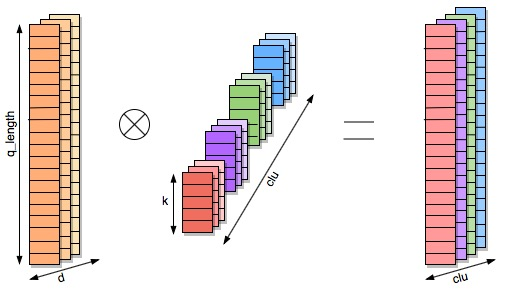
\includegraphics[width=0.8\linewidth]{img/conv1d.jpg}
\end{center}
\caption{The 1-dimensional convolution.}
\label{fig:conv}
\end{figure}
%-------------------------------------------------------------------------
\subsection{CNN Multichannel}    \label{multichannel}
Taking inspiration from \cite{kim2014convolutional}, we investigate a simple modification of the network proposed by \cite{bogdanova2015detecting}. The modified model has two matrices of word embeddings. Each matrix of embeddings is treated as a ‘channel’ and each filter is applied to both channels, but gradients are backpropagated only through one of the channels. Hence the model is able to fine-tune one matrix of embeddings while keeping the other static. Both channels are initialized with pre-trained word embeddings. \\
The outputs of the first hidden layer, in this case, are two matrices $X_0', X_0'' \in \mathbb{R}^{N \times d}$. The matrix $X_0 \in \mathbb{R}^{N \times 2d}$ will be the horizontal concatenation of $X_0'$ and $X_0''$.
  
%------------------------------------------------------------------------
\section{Experiments}

\paragraph{Datasets.}
Our dataset is from Ask Ubuntu Community Questions and Answers site \footnote{http://askubuntu.com}. Ask Ubuntu is a community for Ubuntu users and developers, and it is part of the Stack Exchange Q\&A communities. The users of these communities can ask and answer questions, and vote up and down both questions and answers. Users with high reputation become moderators and can label a new question as a duplicate to an existing question. Usually it takes five votes from different moderators to close a question or to mark it as a duplicate. 
We use Ask Ubuntu data dump \footnote{ \url{https://archive.org/download/stackexchange}} provided in April 2018, that contains posts from 2010 to March 2018. From this data dump we select only the posts that are questions, the amount of questions is $285\,651$. The text of these questions is used for training both the Gensim word2vec model and the CNN. We, then, extract all question pairs linked as duplicated and we assign them a positive label. Since we want to test the performances of our model against the ones obtained by Bogdanova et al., we keep the same dataset size: therefore we consider only $15\,500$ pairs. Finally, we randomly generate the same number of non-duplicated pair of questions (negative samples). \\
The final dataset contains 31K samples and it is perfectly balanced. For our experiments, we divide the data as done in \cite{bogdanova2015detecting}: 24K pairs for the training set, 6K pairs for the test set and 1K pairs for the validation set.

\paragraph{Tokenization.}
Tokenization is the process of breaking up a given text, in this case every question, into units called tokens. The tokens may be words or number or punctuation mark: in this work, we consider only words discarding those tokens that are punctuation, articles and prepositions.
For each word we took only its \emph{lemma}. Lemmatization is a morphological analysis of words, aiming to remove inflectional forms and to return the base or dictionary form of a word, which is known as the \emph{lemma}.

Moreover, we notice that some patterns are very frequent in our text data but not relevant in their different forms. Therefore we take some other precautions:
\begin{itemize}
	\item html tags that are \texttt{code} tags are replaced by the string \texttt{thistokeniscode}
	\item html tags that are \texttt{a} tags are replaced by the string \texttt{thistokenislink}
	\item tokens that match with a time format are replaced by the string \texttt{thistokenistime}
	\item tokens that match with a date format are replaced by the string \texttt{thistokenisdate}
	\item tokens that match with a version format are replaced by the string \texttt{thistokenisversion}
	\item tokens that match with a path format are replaced by the string \texttt{thistokenispath}
	\item tokens that match with a hexadecimal format are replaced by the string \texttt{thistokenishexadecimal}
 \end{itemize}
 
\paragraph{Experiments setup.}
First of all we train the model with pre-trained English Wikipedia's embeddings \footnote{\url{http://nlp.stanford.edu/data/glove.6B.zip}}. In our model we identify the following hyper-parameters: 
\begin{itemize}
	\item $cl_{u}$, that is the number of units of the 1-dimensional convolutional layer
	\item $k$, that is the number of successive words within a window
\end{itemize}
Since the hyper-parameters are continuous and the hyper-parameter space can be very huge, we use a Gaussian Process to approximate the validation accuracy function. At each iteration of this process we sample the hyper-parameters values from Gaussian prior, we train the model with this configuration and we update the Gaussian prior with the validation accuracy of the trained model. Moreover, we use Early Stopping technique to avoid overfitting. \\
After that, in order to evaluate the impact of in-domain word embeddings on the network's performances, we train the model with AskUbuntu embeddings. \\
In both experiments we use Adam optimizer initialized with learning rate $ lr=0.002 $. 


\paragraph{Results and discussion.}
For what concers the issue of unequal text length, the experimental results show that the \emph{max} approach provides the best performances. This is probably due to the fact that the \emph{mean} approach is very likely to drop important semantic information from the sentence. However, it is worth mentioning that, in order for the \emph{max} approach to perform at its best, it is  definitely a good choice dropping the outliers, i.e. the questions that are too long with respect to the other observations. Figure \ref{fig:lens} shows the distribution of the question lengths of our dataset: it is evident that more than 95\% of the questions contains less than 400 words. Hence, we drop the remaining 5\% of the questions.\\
In Figure \ref{fig:wiki}, it is represented the validation accuracy resulted from different combinations of hyper-parameters values. For the sake of clarity, it is shown only the best $cl_{u}$ value for each window size. We observe that increasing too much the number of units of the convolutional layer, $cl_{u}$, provides worst performances. Furthermore, smaller window sizes, provides the best performances.\\
Figure \ref{fig:embeddings} shows that, the addition of a trainable embedding layer, provides a performance improvement of around 1\%. The figure also highlights that (as stated in Table \ref{table:accuracy}) the model trained with in-domain embeddings outperforms that trained using Wikipedia's embeddings.\\
The best model possible is, therefore, the CNN Multi-Channel initialized using in-domain word embeddings with $cl_u=300$ and $k=2$. It achieves 89\% accuracy on the test set.
\begin{table}
\begin{center}
\begin{tabular}{|l|c|}
\hline
Word embedding & Validation accuracy \\
\hline
Wikipedia & 86\% \\
AskUbuntu & 90\% \\
AskUbuntu multichannel & 91\% \\
\hline
\end{tabular}
\end{center}
\caption{Validation Accuracy with word embedding pretrained on different corpora.}
\label{table:accuracy}
\end{table}
\begin{figure}[t]
\begin{center}
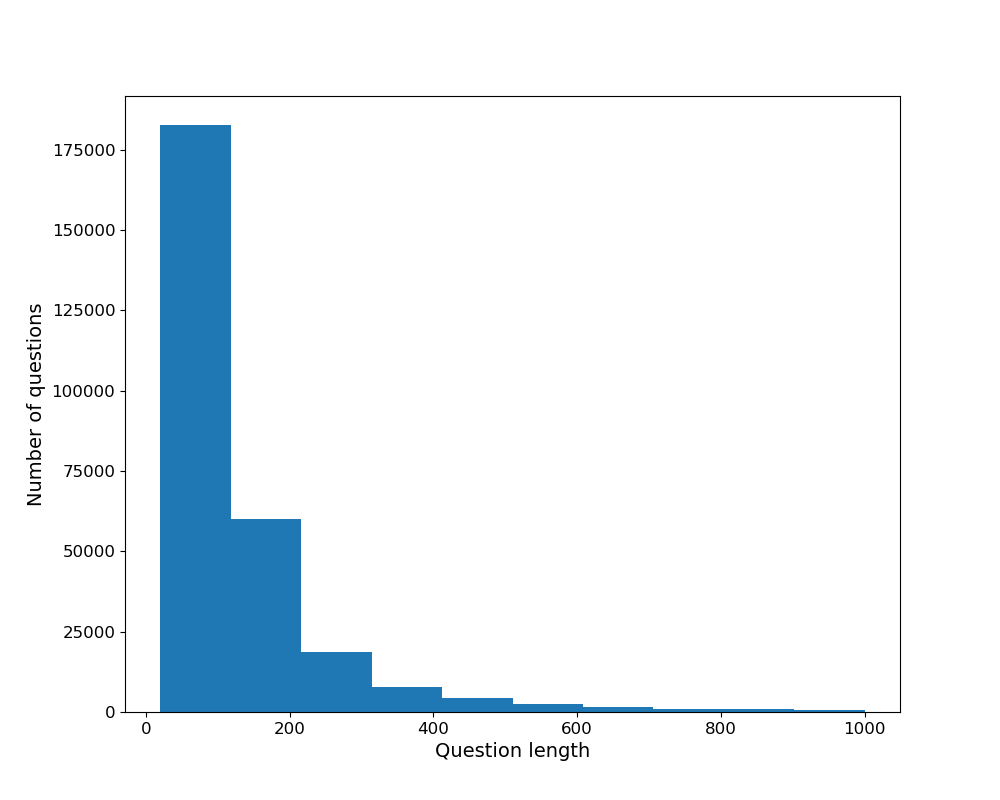
\includegraphics[width=90mm, height= 55mm, scale=1]{img/Histogram.png}
\end{center}
\caption{Distribution of question lengths.}
\label{fig:lens}
\end{figure}
\begin{figure}[t]
\begin{center}
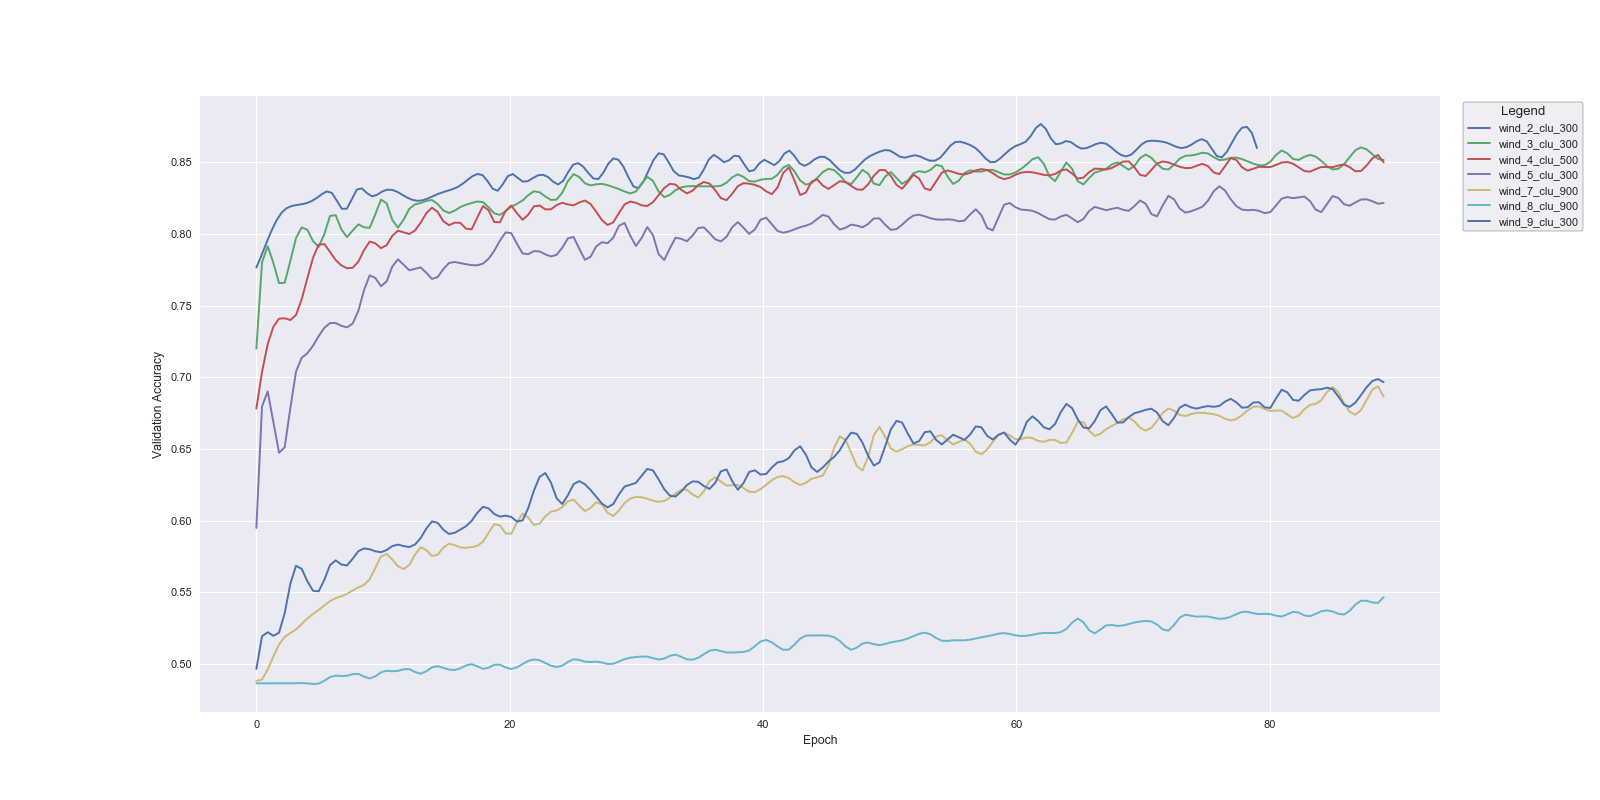
\includegraphics[width=90mm, height= 55mm, scale=1]{img/wiki.png}
\end{center}
\caption{Validation accuracy depending on the hyperparameters.}
\label{fig:wiki}
\end{figure}
\begin{figure}[t]
\begin{center}
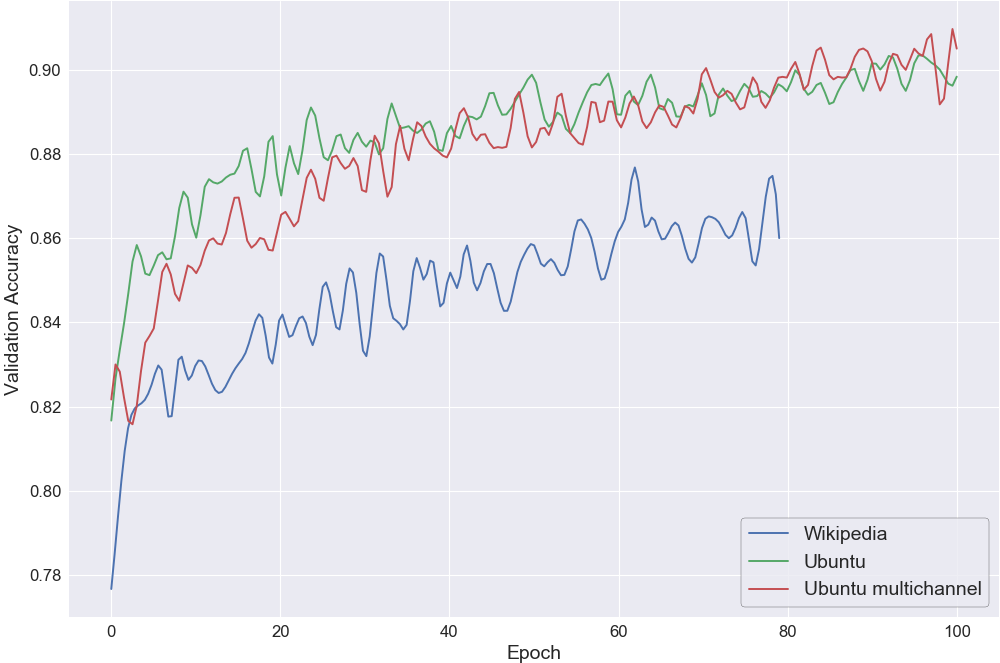
\includegraphics[width=90mm, height= 55mm, scale=1]{img/embeddings_accuracy.png}
\end{center}
\caption{Validation Accuracy using Wikipedia's embeddings, AskUbuntu embeddings and CNN Multi-channel}
\label{fig:embeddings}
\end{figure}

\section{Conclusion} 

In this paper, we attempts to replicate the Bogdonova et al. paper \cite{bogdanova2015detecting}. They propose a method for identifying semantically equivalent questions based on a convolutional neural network. 
We solve the problem of unequal text lengths by choosing the \emph{max} approach, which reaches better performance with respect to the mean approach. We experimentally show that the proposed CNN achieves high accuracy especially when the word embeddings are pre-trained on in-domain data. In particular, we found out that the CNN Multi-channel model brings a performance improvement of one-percent with respect to the model with only one static matrix of word embeddings . This model achieves 89\% accuracy on the test set, that is a result very close to the one of our target.\\
A possible extension of this work could be to use an LSTM approach to solve the problem of unequal text lengths. Moreover, other deeper architectures could be investigated.

%-------------------------------------------------------------------------



{\small
\bibliographystyle{ieee}
\bibliography{bib}
}

\end{document}
